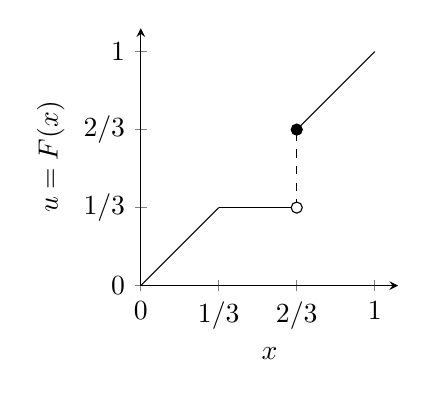
\begin{tikzpicture}
    \begin{axis}[
    axis lines=left,
    xlabel = $x$, ylabel = {$u = F(x)$},
    xmax = 1.1, xtick = {0, 1/3, 2/3, 1}, 
    ymax = 1.1, ytick = {0, 1/3, 2/3, 1},
    xticklabels={$0$, $1/3$, $2/3$, $1$},
    yticklabels={$0$, $1/3$, $2/3$, $1$}, 
    width=0.4\textwidth, height=0.4\textwidth]
    \addplot[domain=0:1/3] {x};
    \addplot[domain=1/3:2/3] {1/3};
    \addplot[domain=2/3:1] {x};
    \addplot[mark=*,only marks] coordinates {(2/3,2/3)};
    \addplot[mark=*,fill=white,only marks] coordinates {(2/3,1/3)};
    \draw [dashed] (2/3,1/3) -- (2/3,2/3);
    \end{axis}
\end{tikzpicture}